\documentclass{beamer}
\usepackage{tikz}
\newcommand{\zcb}[1]{#1\text{-yr}}
\renewcommand{\arraystretch}{1.5}
\newcommand{\should}{\overset{\text{should}}{=}}
\newcommand{\fttheory}[1]{\fcolorbox{blue}{blue}{\color{white}\textbf{#1}\hspace{\textwidth}}}
\newcommand{\ftexampl}[1]{\fcolorbox{orange}{orange}{\color{black}\textbf{#1}\hspace{\textwidth}}}
\newcommand{\ftdata}[1]{\fcolorbox{violet}{violet}{\color{white}\textbf{#1}\hspace{\textwidth}}}
\newcommand{\ftheader}[1]{\fcolorbox{lightgray}{lightgray}{\color{black}\textbf{#1}\hspace{\textwidth}}}
\begin{document}

\begin{frame}{\ftheader{Bond Prices, Yields, and Arbitrage}}
	\begin{itemize}
		\item We're going to study the \underline{yield curve}
		\item Specifically, we're going to study
		\begin{enumerate}
			\item What the yield curve can tell us about the economy
			\item What current yields tell us about future yields
			\item How to price bonds using the yield curve
		\end{enumerate}
	\end{itemize}
\end{frame}

\begin{frame}{\fttheory{Arbitrage}}
	\begin{itemize}
		\item Consider a 1-year, 100 USD, zero-coupon bond that compounds annually
		\item Suppose that you can borrow and lend for 1 year at 10\% (which compounds annually)
		\item Now
		\begin{equation}
			p_{0}\overset{\text{``should''}}{=}\frac{100\text{ USD}}{1+0.1}=90.9091
		\end{equation}
		\item Suppose that $p_{0}\overset{\text{``actual''}}{=}100$. 
	\end{itemize}
\end{frame}

\begin{frame}{Arbitrage}
	\begin{itemize}
		\item Suppose that $p_{0}\overset{\text{``actual''}}{=}90$. 
		\begin{center}
		\begin{tabular}{l|rr}
			\textbf{Security} & \textbf{CF}$_{0}$ & \textbf{CF}$_{1}$ \\ \hline
			Bond & $-90.0000$ & +100\\
			Borrow & $+90.9091$ & -100\\ \hline
				& $+0.9091$ & 0
		\end{tabular}
		\end{center}
		\item On date 0 (today), borrow 90.9091 USD, use 90 of it to buy the bond, pocket the .9091. On date 1 (in one year), collect the 100 from the bond and use it to pay off your loan.
	\end{itemize}
\end{frame}

\begin{frame}{Arbitrage}
	\begin{itemize}
		\item Suppose that $p_{0}\overset{\text{``actual''}}{=}91$. 
		\begin{center}
		\begin{tabular}{l|rr}
			\textbf{Security} & \textbf{CF}$_{0}$ & \textbf{CF}$_{1}$ \\ \hline
			Bond & $+91.0000$ & -100\\
			Lend & $-90.9091$ & +100\\ \hline
				& $0.9091$ & 0
		\end{tabular}
		\end{center}
		\item On date 0 (today), short the bond, collect 91 USD, lend 90.9091 of it, and pocket the .9091. On date 1 (in one year), collect the 100 USD from your loan and pay 100 to the person whose bond you shorted.
	\end{itemize}
\end{frame}

\begin{frame}
	\begin{itemize}
		\item These portfolios were ``free'' in the sense that they did not require any up-front capital
		\item If one trader observes the mispricing, she will be able to exploit it and earn arbitrage profits
		\item As more and more traders enter the market to buy (or sell) the bond, the price converges to its ``should'' price
	\end{itemize}
\end{frame}

\section{Yield Curve}
\begin{frame}
	\begin{itemize}
		\item For each term (e.g. 1 month, 1 year, 30 years), the yield curve tells us the yield of the corresponding zero-coupon bond
		\item Example 1: if the 10-year yield is 1.61\% (as read from the yield curve), then a 10-year zero coupon bond should have yield 1.61\% and should trade for
			\begin{equation}
				P=\frac{100\text{ USD }}{1+10\times0.0161}=86.1326\text{ USD}
			\end{equation}
		\item It is \underline{not} the yield on a 10-year Treasury note (because the note's yield depends on its coupon rate)
		\item Example 2: if the 1-month yield is 1.55\% (as read from the yield curve), then a 1-month zero coupon bond should have yield 1.55\% and should trade for
			\begin{equation}
				P=\frac{100\text{ USD }}{1+0.0155/12}=99.8710\text{ USD}
			\end{equation}
	\end{itemize}
\end{frame}

\begin{frame}{A typical yield curve}
\begin{center}
	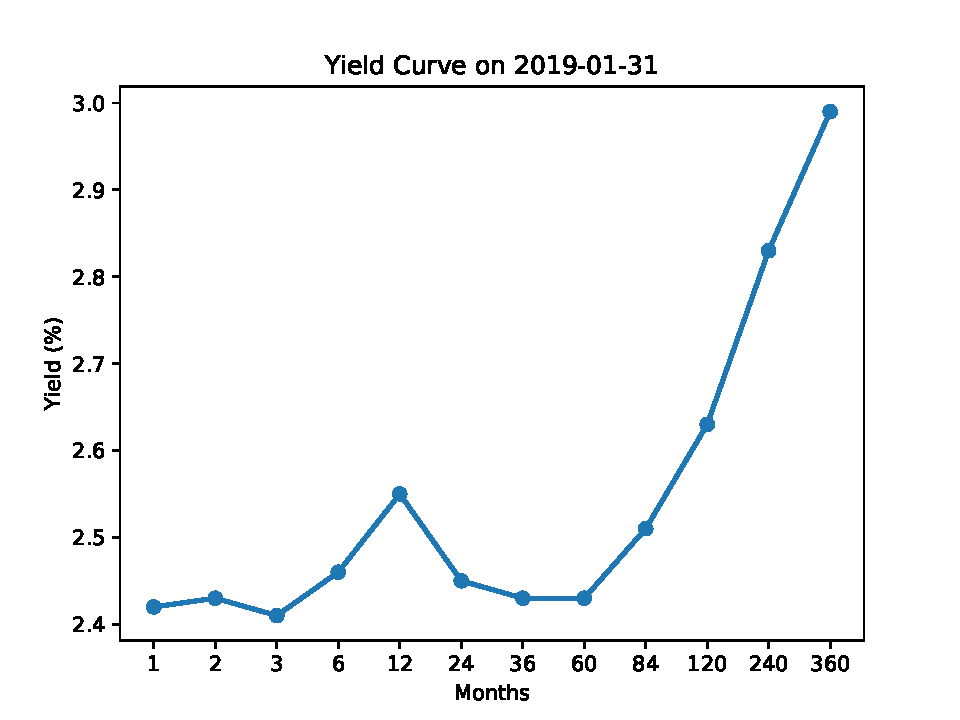
\includegraphics[scale=.55]{xs20190131}
\end{center}
\end{frame}

\begin{frame}{Entering recession}
	\begin{center}
		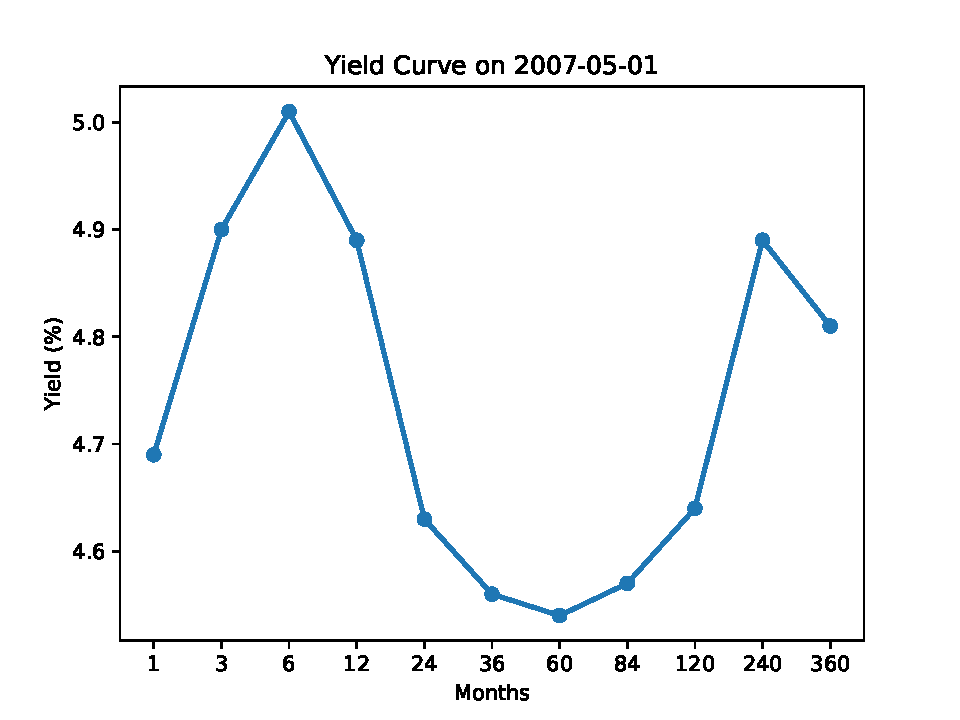
\includegraphics[scale=.55]{xs20070501}
	\end{center}
\end{frame}

\begin{frame}{Why are there different rates?} 
	\begin{itemize}
		\item Why are there different rates? Why isn't there just one rate for all terms?
		\item The shape of the yield curve is pinned-down by something called a \emph{stochatic discount factor}, the discussion of which is beyond the scope of this course\footnote{The interested student should study \textit{Optimal Control Theory}}
		\item When conditions are expected to improve, the curve is upward sloping; when they are expected to deteriorate, the curve is downward sloping
		\item Application: banks borrow short and lend long
	\end{itemize}
\end{frame}

\begin{frame}{In the time-series...}
\begin{center}
	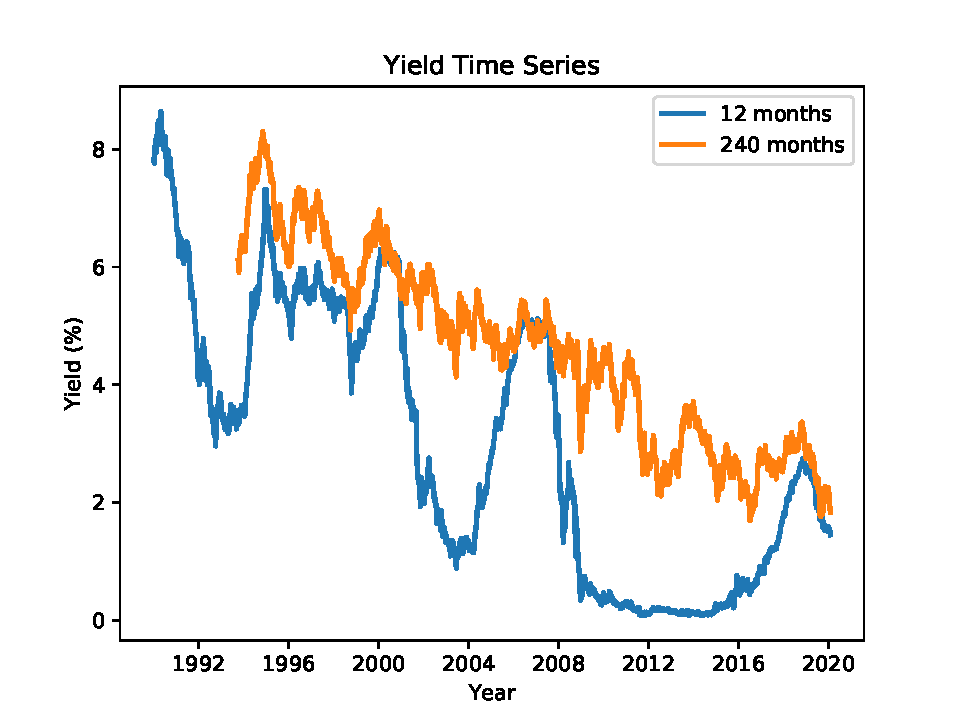
\includegraphics[scale=.55]{ts12240}
\end{center}
\end{frame}

% Reference
\iffalse
\begin{frame}{Forward Rates (Reference)}
	\small
	\begin{figure}[H]
		\begin{center}
			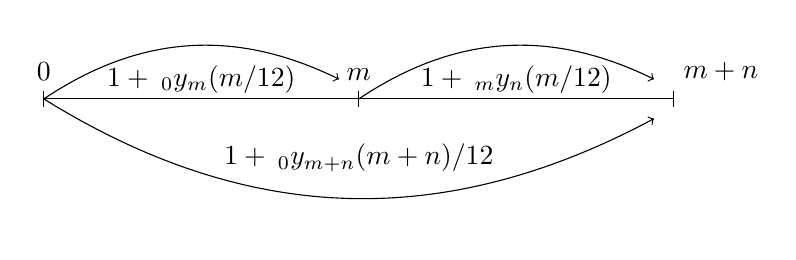
\begin{tikzpicture}
				\draw (0,0) -- (8,0);
				\foreach \x in {0,4,8}
				\draw(\x cm,3pt) -- (\x cm, -3pt);
				\draw (0,0) node[above=3pt] {0};
				\draw (4,0) node[above=3pt] {$m$};
				\draw (8,0) node[above=3pt,anchor=south west] {$m+n$};
				\draw[->] (0,0) to[bend left] (3.75,.25);
				\draw[->] (4,0) to[bend left] (7.75,.25);
				\draw[->] (0,0) to[bend right] (7.75,-.25);
				\draw (2,.25) node{$1+\:_{0}y_{m}(m/12)$};
				\draw (6,.25) node{$1+\:_{m}y_{n}(m/12)$};
				\draw (4,-.75) node{$1+\:_{0}y_{m+n}(m+n)/12$};
			\end{tikzpicture}
		\end{center}
	\end{figure}
	\vfill
	\begin{itemize}
		\item $_{0}y_{m}$ is the yield today (date 0) on a $m$-month zero coupon bond that matures in $m$ months (date $m$)
		\item $_{0}y_{m+n}$ is the yield today (date 0) on a $m+n$-month zero coupon bond that matures in $m+n$ months (date $m+n$)
		\item $_{m}y_{n}$ is the yield in $m$ months (date $m$) on a $n$-month zero coupon bond that matures in $m+n$ months (date $m+n$)
	\end{itemize}
\end{frame}

% A Multiyear Investor
\begin{frame}{Forward Rates (Reference)}
	\small
	\begin{figure}[H]
		\begin{center}
			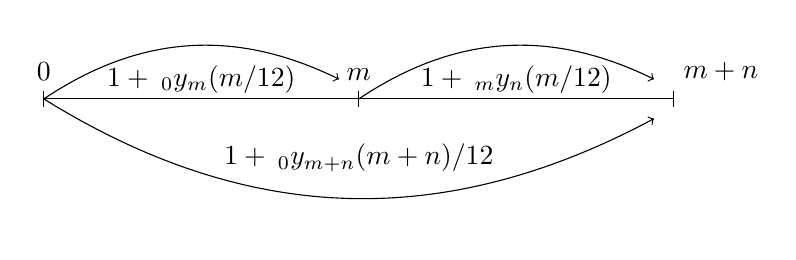
\begin{tikzpicture}
				\draw (0,0) -- (8,0);
				\foreach \x in {0,4,8}
				\draw(\x cm,3pt) -- (\x cm, -3pt);
				\draw (0,0) node[above=3pt] {0};
				\draw (4,0) node[above=3pt] {$m$};
				\draw (8,0) node[above=3pt,anchor=south west] {$m+n$};
				\draw[->] (0,0) to[bend left] (3.75,.25);
				\draw[->] (4,0) to[bend left] (7.75,.25);
				\draw[->] (0,0) to[bend right] (7.75,-.25);
				\draw (2,.25) node{$1+\:_{0}y_{m}(m/12)$};
				\draw (6,.25) node{$1+\:_{m}y_{n}(m/12)$};
				\draw (4,-.75) node{$1+\:_{0}y_{m+n}(m+n)/12$};
			\end{tikzpicture}
		\end{center}
	\end{figure}
	\vfill
	\begin{equation}
		(1+\:_{0}y_{1}(m/12)(1+\:_{1}y_{1}(n/12)\should1+\:_{0}y_{2}/6. 
	\end{equation}
	\begin{itemize}
		\item The current yield curve ($_{0}y_{1},_{0}y_{2}$) predicts the future short-term yield ($_{1}y_{1}$), which we call the \textit{forward rate}
		\item This relationship between current and future yields is known as the \emph{expectations hypothesis}
	\end{itemize}
\end{frame}
\fi

% A Multiyear Investor
\begin{frame}{Forward Rates (One-Month)}
	\begin{figure}[H]
		\begin{center}
			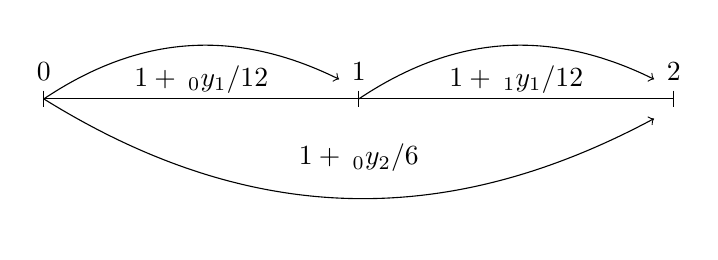
\begin{tikzpicture}
				\draw (0,0) -- (8,0);
				\foreach \x in {0,4,8}
				\draw(\x cm,3pt) -- (\x cm, -3pt);
				\draw (0,0) node[above=3pt] {0};
				\draw (4,0) node[above=3pt] {1};
				\draw (8,0) node[above=3pt] {2};
				\draw[->] (0,0) to[bend left] (3.75,.25);
				\draw[->] (4,0) to[bend left] (7.75,.25);
				\draw[->] (0,0) to[bend right] (7.75,-.25);
				\draw (2,.25) node{$1+\:_{0}y_{1}/12$};
				\draw (6,.25) node{$1+\:_{1}y_{1}/12$};
				\draw (4,-.75) node{$1+\:_{0}y_{2}/6$};
			\end{tikzpicture}
		\end{center}
	\end{figure}
	\vfill
	{\small
	\begin{itemize}
		\item $_{0}y_{1}$ is the yield today (date 0) on a 1-month zero coupon bond that matures in one month (date 1)
		\item $_{0}y_{2}$ is the yield today (date 0) on a 2-month zero coupon bond that matures in two months (date 2)
		\item $_{1}y_{1}$ is the yield in one month (date 1) on a 1-month zero coupon bond that matures in two months (date 2)
	\end{itemize}
	}
\end{frame}

% A Multiyear Investor
\begin{frame}{Forward Rates (One-Month)}
	\begin{figure}[H]
		\begin{center}
			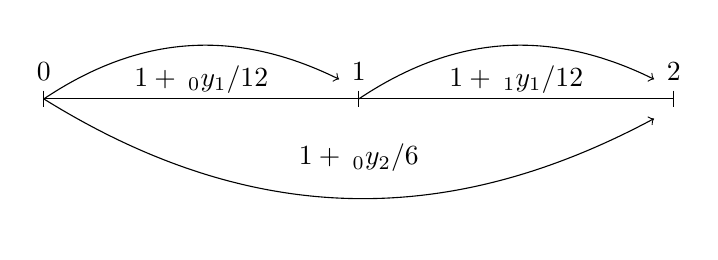
\begin{tikzpicture}
				\draw (0,0) -- (8,0);
				\foreach \x in {0,4,8}
				\draw(\x cm,3pt) -- (\x cm, -3pt);
				\draw (0,0) node[above=3pt] {0};
				\draw (4,0) node[above=3pt] {1};
				\draw (8,0) node[above=3pt] {2};
				\draw[->] (0,0) to[bend left] (3.75,.25);
				\draw[->] (4,0) to[bend left] (7.75,.25);
				\draw[->] (0,0) to[bend right] (7.75,-.25);
				\draw (2,.25) node{$1+\:_{0}y_{1}/12$};
				\draw (6,.25) node{$1+\:_{1}y_{1}/12$};
				\draw (4,-.75) node{$1+\:_{0}y_{2}/6$};
			\end{tikzpicture}
		\end{center}
	\end{figure}
	\vfill
	\begin{equation}
		(1+\:_{0}y_{1}/12)(1+\:_{1}y_{1}/12)\should1+\:_{0}y_{2}/6. 
	\end{equation}
	{\small
	\begin{itemize}
		\item The current yield curve ($_{0}y_{1},_{0}y_{2}$) predicts the future short-term yield ($_{1}y_{1}$), which we call the \textit{forward rate}
		\item This relationship between current yields and future yields is called the \textit{expectations hypothesis}
	\end{itemize}
	}
\end{frame}
\begin{frame}{Forward Rates}
$_0y_1=1.57\%$ and $_0y_2=1.58\%$. Is the market optimistic or pessimistic about the economy (in the short-term)? What did the market expect the 1-month yield to be in one month ($_1y_1$)?
	\pause
	{\color{blue}
		\begin{equation}
			_{1}y_{1}=12\left(\frac{1+_0y_2/6}{1+_0y_1/12}-1\right)=1.5879\%
		\end{equation}
	}
\end{frame}

\begin{frame}{\ftexampl{Forward Rates}}
On 2019-01-01, $_0y_1=2.40\%$ and $_0y_2=2.40\%$. What did the market expect the 1-month yield to be in one month ($_1y_1$)?
	\pause
	{\color{blue}
		\begin{equation}
			_{1}y_{1}=12\left(\frac{1+_0y_2/6}{1+_0y_1/12}-1\right)=2.3952\%
		\end{equation}
	}
\end{frame}

\iffalse
% A Multiyear Investor
\begin{frame}{Forward Rates: Two-Month}
	\begin{figure}[H]
		\begin{center}
			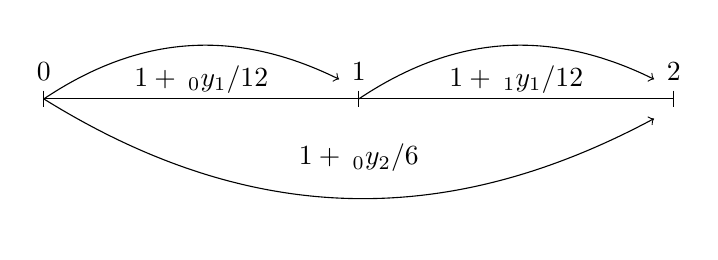
\begin{tikzpicture}
				\draw (0,0) -- (8,0);
				\foreach \x in {0,4,8}
				\draw(\x cm,3pt) -- (\x cm, -3pt);
				\draw (0,0) node[above=3pt] {0};
				\draw (4,0) node[above=3pt] {1};
				\draw (8,0) node[above=3pt] {2};
				\draw[->] (0,0) to[bend left] (3.75,.25);
				\draw[->] (4,0) to[bend left] (7.75,.25);
				\draw[->] (0,0) to[bend right] (7.75,-.25);
				\draw (2,.25) node{$1+\:_{0}y_{1}/12$};
				\draw (6,.25) node{$1+\:_{1}y_{1}/12$};
				\draw (4,-.75) node{$1+\:_{0}y_{2}/6$};
			\end{tikzpicture}
		\end{center}
	\end{figure}
	\vfill
	\begin{equation}
		(1+\:_{0}y_{1}/12)(1+\:_{1}y_{1}/12)\should1+\:_{0}y_{2}/6. 
	\end{equation}
	\begin{itemize}
		\item The current yield curve ($_{0}y_{1},_{0}y_{2}$) predicts the future short-term yield ($_{1}y_{1}$), which we call the \textit{forward rate}
	\end{itemize}
\end{frame}

\begin{frame}{Forward Rates}
$_0y_1=1.57\%$ and $_0y_3=1.56. $Is the market optimistic or pessimistic about the economy (in the short-term)? What does the market expect the 2-month yield to be in one month ($_1y_2$)?
	\pause
	{\color{blue}
		\begin{equation}
			_{1}y_{2}=
		\end{equation}
	}
\end{frame}

% A Multiyear Investor
\begin{frame}{Forward Rates: Two-Month}
	\begin{figure}[H]
		\begin{center}
			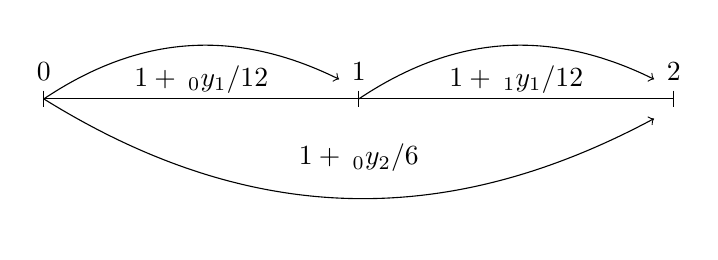
\begin{tikzpicture}
				\draw (0,0) -- (8,0);
				\foreach \x in {0,4,8}
				\draw(\x cm,3pt) -- (\x cm, -3pt);
				\draw (0,0) node[above=3pt] {0};
				\draw (4,0) node[above=3pt] {1};
				\draw (8,0) node[above=3pt] {2};
				\draw[->] (0,0) to[bend left] (3.75,.25);
				\draw[->] (4,0) to[bend left] (7.75,.25);
				\draw[->] (0,0) to[bend right] (7.75,-.25);
				\draw (2,.25) node{$1+\:_{0}y_{1}/12$};
				\draw (6,.25) node{$1+\:_{1}y_{1}/12$};
				\draw (4,-.75) node{$1+\:_{0}y_{2}/6$};
			\end{tikzpicture}
		\end{center}
	\end{figure}
	\vfill
	\begin{equation}
		(1+\:_{0}y_{1}/12)(1+\:_{1}y_{1}/12)\should1+\:_{0}y_{2}/6. 
	\end{equation}
	\begin{itemize}
		\item The current yield curve ($_{0}y_{1},_{0}y_{2}$) predicts the future short-term yield ($_{1}y_{1}$), which we call the \textit{forward rate}
	\end{itemize}
\end{frame}
\fi

%-----------------------------------------------------------------------------%
% BOND PRICES
%-----------------------------------------------------------------------------%
\section{Prices}

% Annuities
\begin{frame}{Coupon Bonds}
	We can use the yield curve to compute the price of a coupon bond. A $T$-year coupon bond makes annual payments
	\begin{figure}[H]
		\begin{center}
			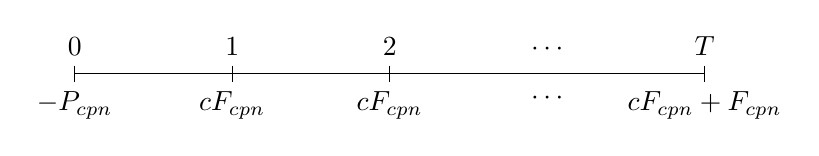
\begin{tikzpicture}
				\draw (0,0) -- (8,0);
				\foreach \x in {0,2,4,8}
				\draw(\x cm,3pt) -- (\x cm, -3pt);
				\draw (0,0) node[above=3pt] {0};
				\draw (2,0) node[above=3pt] {1};
				\draw (4,0) node[above=3pt] {2};
				\draw (8,0) node[above=3pt] {$T$};
				\draw (0,0) node[below=3pt] {$-P_{\text{cpn}}$};
				\draw (2,0) node[below=3pt] {$cF_{\text{cpn}}$};
				\draw (4,0) node[below=3pt] {$cF_{\text{cpn}}$};
				\draw (6,0) node[above=3pt, align=center] {$\cdots$};
				\draw (6,0) node[below=3pt, align=center] {$\cdots$};
				\draw (8,0) node[below=3pt] {$cF_{\text{cpn}}+F_{\text{cpn}}$};
			\end{tikzpicture}
		\end{center}
	\end{figure}
where $c\geq0$ is the coupon rate (APR) and $F_{\text{cpn}}$ is the face value of the coupon bond
\begin{align*}
	P_{\text{cpn}}&\should \left[\frac{cF_{\text{cpn}}}{F_{\zcb{1}}}\right]P_{\zcb{1}}+\left[\frac{cF_{\text{cpn}}}{F_{\zcb{1}}}\right]P_{\zcb{2}}+\cdots+\left[\frac{(1+c)F_{\text{cpn}}}{F_{\zcb{T}}}\right]P_{\zcb{T}}
\end{align*}
where $y$ is the yield (APR) and $P_{\zcb{k}}$ is the price of a $k$-year zero coupon bond with face value of $F_{\zcb{k}}$
\end{frame}

\begin{frame}{\ftexampl{Example}}
	\small
	What is the price of a 3-year, 1000 USD 10\% coupon bond that makes payments annual coupon payments. The 1-year yield is 1.48\%, the 2-year yield is 1.41\%, and the 3-year yield is 1.40\%. What should the 3-year \textit{coupon} bond trade for?
	\pause
	{\color{blue}
		First, compute the prices of the zero-coupon bonds:
		\begin{align}
			p_{1}&=\frac{100\text{ USD}}{1+1\times0.0148}=98.5416\text{ USD}\\
			p_{2}&=\frac{100\text{ USD}}{1+2\times0.0141}=97.2373\text{ USD}\\
			p_{3}&=\frac{100\text{ USD}}{1+3\times0.0140}=95.9693\text{ USD}
		\end{align}	
		Next, note that the cash-flows from the zero coupon bond are 100 USD, 100 USD, and 1100 USD.
		\begin{equation}
			p_{\text{cpn}}=1\times p_{1}+1\times p_{2}+11\times p_{3}=1251.4612\text{ USD}
		\end{equation}
	}
\end{frame}
\begin{frame}{\ftexampl{Example}}
	\small
	What is the price of a 3-year, 1000 USD 5\% coupon bond that makes payments annual coupon payments. The 1-year yield is 1.59\%, the 2-year yield is 1.58\%, and the 3-year yield is 1.62\%. What should the 3-year \textit{coupon} bond trade for?
	\pause
	{\color{blue}
		First, compute the prices of the zero-coupon bonds:
		\begin{align}
			p_{1}&=\frac{100\text{ USD}}{1+1\times0.0159}=98.4349\text{ USD}\\
			p_{2}&=\frac{100\text{ USD}}{1+2\times0.0158}=96.9368\text{ USD}\\
			p_{3}&=\frac{100\text{ USD}}{1+3\times0.0162}=95.3652\text{ USD}
		\end{align}	
		Next, note that the cash-flows from the zero coupon bond are 50 USD, 50 USD, and 1050 USD.
		\begin{equation}
			p_{\text{cpn}}=\frac{1}{2}\times p_{1}+\frac{1}{2}\times p_{2}+\left(10+\frac{1}{2}\right)\times p_{3}=1099.0205\text{ USD}
		\end{equation}
	}
\end{frame}

\begin{frame}{\ftheader{Yield-to-Maturity}}
	\begin{itemize}
		\item In our previous lectures, we saw that market participants borrow/lend at different yields \textit{depending on the term}  
		\item Rather than carry around an entire yield curve whenever we want to recompute the price of a bond, we summarize this information with the \textit{yield-to-maturity} (YTM), with which you are familiar from your previous coursework
		\item Example: consider a 1000 USD, 30-year, 5\% T-bond that makes semi-annual payments, and trades for 1011.9610 USD 
		\item The YTM on this T-bond is the \underline{one} rate that would make the PV of cash-flows equal to the price, namely, 4.9233\%
	\end{itemize}
\end{frame}

\begin{frame}{\ftexampl{YTM Example}}
		Suppose that 1, 2, and 3-year, 100 USD zero-coupon bonds trade for 106.4607, 99.7684, and 93.7438 USD respectively. What should be the YTM of a 3-year, 1000 USD, 10\% coupon bond that makes annual payments? \\
		\pause
	{\color{blue}

		First compute what the price should be.
		\begin{equation*}
			p_{\text{cpn}}\should 1\times106.4607+1\times99.7684+11\times93.7438=1237.4109\text{ USD}
		\end{equation*}
		Then we can compute the YTM using a financial calculator: NPER $=$ 3, PMT $=$ 100 USD, PV $=$ 1237.4109 USD, and FV $=$ 1000 gives us a YTM of 1.7998\%.
	}
\end{frame}

\end{document}
